\documentclass[letter,11pt]{article}
\usepackage[breaklinks]{hyperref}
\hypersetup{
    bookmarks=true,         % show bookmarks bar?
    unicode=false,          % non-Latin characters in Acrobat’s bookmarks
    pdftoolbar=true,        % show Acrobat’s toolbar?
    pdfmenubar=true,        % show Acrobat’s menu?
    pdffitwindow=false,     % window fit to page when opened
    pdfstartview={XYZ null null 1.00},    % disable zoom
    pdftitle={Linux @ UMBC},    % title
    pdfauthor={Richard Zak},     % author
    pdfsubject={Linux @ UMBC},   % subject of the document
    pdfkeywords={Computer Science, Programming, Linux, UMBC, CSEE}, % list of keywords
    pdfnewwindow=true,      % links in new PDF window
    colorlinks=false,       % false: boxed links; true: colored links
    linkcolor=red,          % color of internal links (change box color with linkbordercolor)
    citecolor=green,        % color of links to bibliography
    filecolor=magenta,      % color of file links
    urlcolor=cyan           % color of external links
}
\usepackage{graphicx}
\usepackage{placeins}
\usepackage{fancyhdr}
\usepackage{multicol}
\pagestyle{fancy}
\usepackage[letterpaper, margin=1in]{geometry}
\geometry{letterpaper}
\usepackage{parskip} % Disable initial indent
\usepackage{color,soul} % Highligher
\usepackage[normalem]{ulem} % Strikethrough with \sout{}

\usepackage[utf8]{inputenc}
\fancyhf{}
\renewcommand{\headrulewidth}{0pt} % Remove default underline from header package
\rhead{Connecting to and Using UMBC's Linux Servers\begin{picture}(0,0) \put(85,-6){
\includegraphics[width=1.1cm]{Images/Tux.png}} \end{picture}}
%\rhead{}
\lhead{\begin{picture}(0,0) \put(0,-10){
\includegraphics[width=1.1cm]{Images/UMBC-vertical}} \end{picture}}
\cfoot{\thepage}
\rfoot{}
\lfoot{Linux @ UMBC}
\AtEndDocument{\vfill \footnotesize{Last updated 22 Aug 2020} \hfill \LaTeX}

\begin{document}

\section{Windows Users}
\FloatBarrier
\subsection{Putty}
\paragraph{}Putty is a Windows program which provides access to the command line interface on a UNIX system, which includes Linux. It's not the only program which can be used for this, but it's the easiest to use and most convenient.

\begin{enumerate}
    \item Start by downloading Putty from \url{https://www.chiark.greenend.org.uk/~sgtatham/putty/latest.html}. The Installer option adds the option to have a shortcut on the desktop. However, the \texttt{putty.exe} link under ``Alternative binary files'' provides the program itself, which you may place where you'd like.
    \item When you launch Putty, enter \texttt{gl.umbc.edu} in the ``Host Name'' field and click ``Open'', as shown in \autoref{fig:puttyconnection}.
    \item For the first time you connect, you'll see a box asking about caching the host key. Don't worry about this, click ``Yes'', as shown in \autoref{fig:puttyserverkey}.
    \item A black window will appear asking for your user name, then you'll see some text from UMBC, followed by a password prompt. Type your password, and it will not be shown. \autoref{fig:puttyconnected} shows what you'll see once connected.
\end{enumerate}

\begin{figure}
\centering
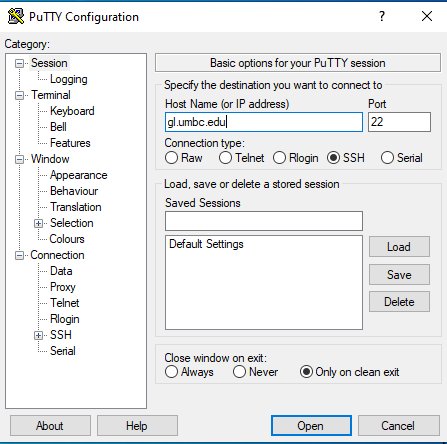
\includegraphics[scale=0.6]{Images/putty_connect_1.png}
\caption{The Putty connection dialog box.}
\label{fig:puttyconnection}
\end{figure}

\begin{figure}
\centering
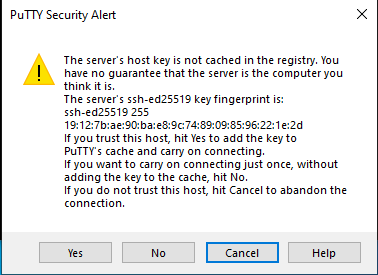
\includegraphics[scale=0.7]{Images/putty_connect_2_first_time.png}
\caption{Putty asking about the server SSH key.}
\label{fig:puttyserverkey}
\end{figure}

\begin{figure}
\centering
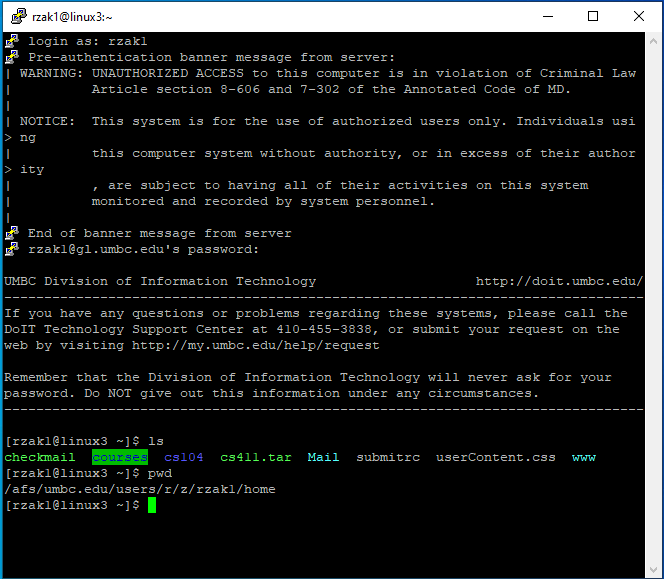
\includegraphics[scale=0.7]{Images/putty_connected.png}
\caption{Putty is connected to the Linux server.}
\label{fig:puttyconnected}
\end{figure}

\FloatBarrier
\subsection{WinSCP}
\paragraph{}Putty allows you to enter commands on the Linux command line interface, and WinSCP allows you to transfer files to and from the Linux environment using the familiar drag-and-drop interface.

\begin{enumerate}
    \item Start by downloading WinSCP from \url{https://winscp.net/eng/download.php}, which provides the installer. If you want to have a portable version which you can place anywhere, visit \url{https://winscp.net/eng/downloads.php}.
    \item Launch WinSCP and enter \texttt{gl.umbc.edu} in the ``Host name'' field, your user name \& password in the appropriate fields. Click ``Login''. An example is shown in \autoref{fig:winscpconnect}.
    \item Just as with Putty, the first time you connect, you'll be asked to accept the server's SSH key. Click ``Yes'', as shown in \autoref{fig:winscpconnectfirsttime}.
    \item Once connected, you'll see a two-pane window showing your local computer on the left, and the files \& directories (folders) on the right, as shown in \autoref{fig:winscpconnected}.
\end{enumerate}

\begin{figure}
\centering
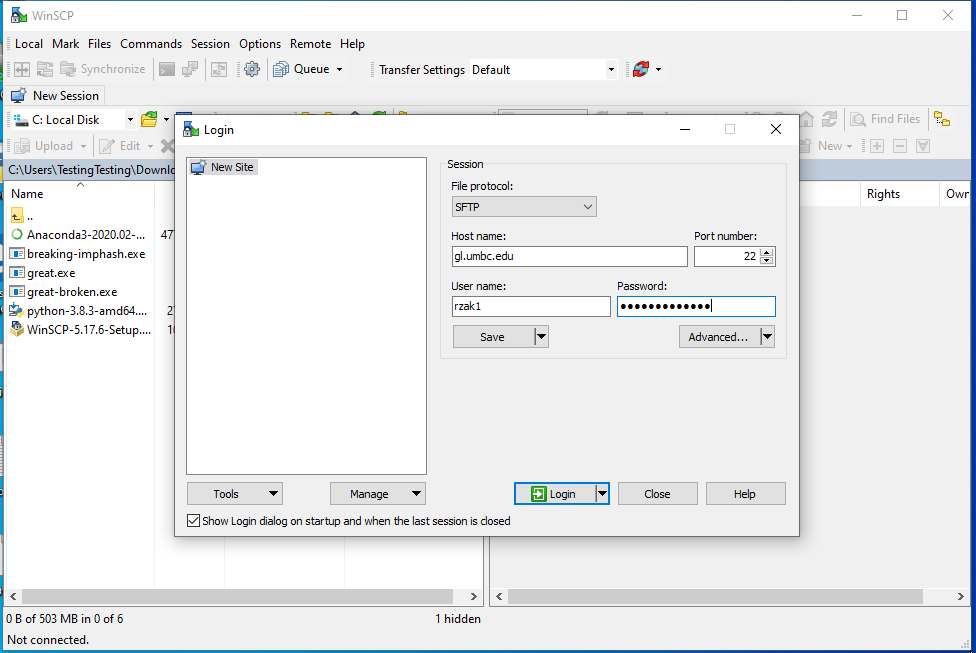
\includegraphics[scale=0.6]{Images/winscp_gl_connect.png}
\caption{WinSCP connection dialog box.}
\label{fig:winscpconnect}
\end{figure}

\begin{figure}
\centering
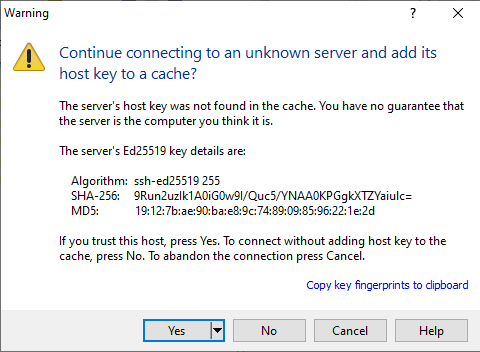
\includegraphics[scale=0.7]{Images/winscp_connect_first_time.png}
\caption{WinSCP asking about the server SSH key.}
\label{fig:winscpconnectfirsttime}
\end{figure}

\begin{figure}
\centering
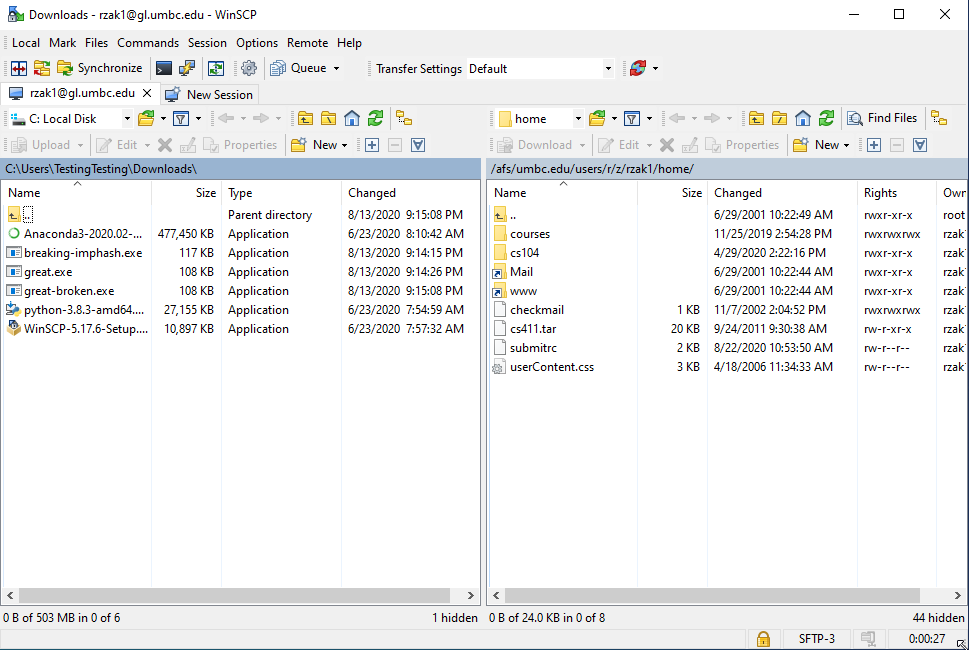
\includegraphics[scale=0.6]{Images/winscp_connected.png}
\caption{WinSCP showing local and remote files.}
\label{fig:winscpconnected}
\end{figure}

\FloatBarrier
\section{Mac Users}
\subsection{Terminal.app}
\paragraph{}The Mac operating system comes from a strong UNIX legacy. As such, the required components to interact with Linux servers at UMBC are already installed and ready to go! You'll use the Terminal application to connect to UMBC's servers. You can easily find the Terminal by navigating to Applications $\,\to\,$ Utilities, as shown in \autoref{fig:macfinderterminal} or by using Spotlight by pressing 
\includegraphics[height=.75em]{Images/command.eps} Space and begin typing Terminal, as shown in \autoref{fig:macspotlightterminal}.

\paragraph{}Once Terminal is open, type: \texttt{ssh userName@gl.umbc.edu} and press enter. Enter your password when prompted, and note that the password is shown. An example is shown in \autoref{fig:macterminalconnected}. For convenience, you can keep the Terminal icon in the Dock for future use. Right-Click on the Terminal icon, select Options $\,\to\,$ Keep in Dock, as shown in \autoref{fig:macterminaldock}.

\begin{figure}
\centering
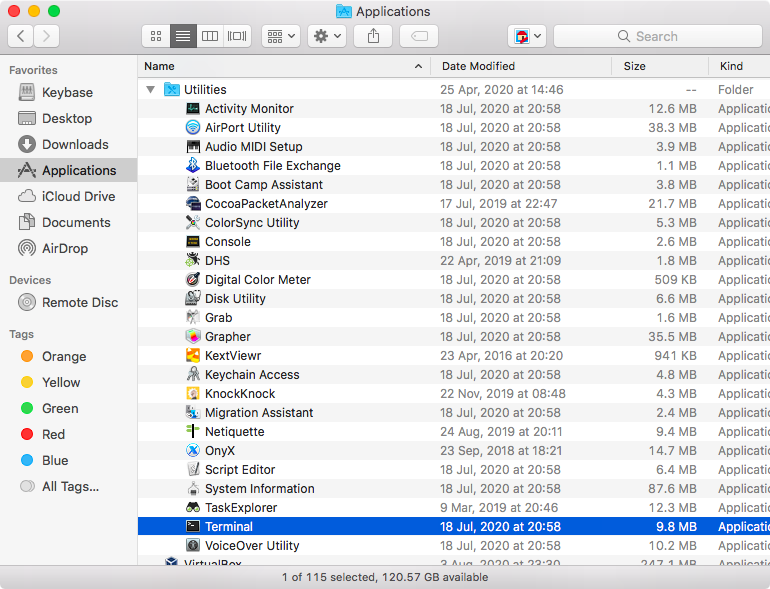
\includegraphics[scale=0.6]{Images/finder_terminal.png}
\caption{Finding Terminal with Finder.}
\label{fig:macfinderterminal}
\end{figure}

\begin{figure}
\centering

\includegraphics[scale=0.6]{Images/spotlight_terminal.png}
\caption{Searching for Terminal with Spotlight.}
\label{fig:macspotlightterminal}
\end{figure}

\begin{figure}
\centering
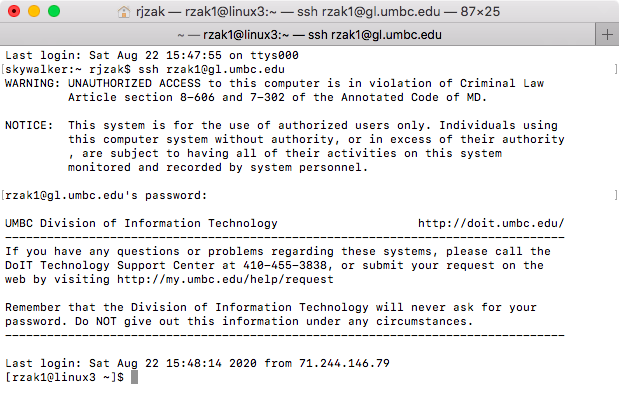
\includegraphics[scale=0.6]{Images/macos_terminal_ssh.png}
\caption{Terminal showing the SSH connection.}
\label{fig:macterminalconnected}
\end{figure}

\begin{figure}
\centering
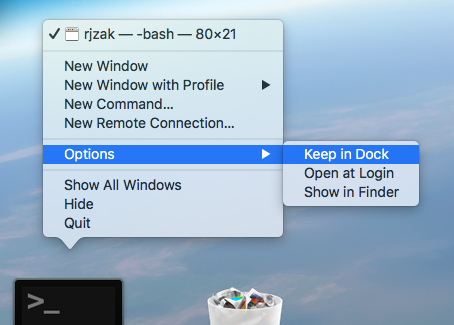
\includegraphics[scale=0.6]{Images/terminal_keep_in_dock.png}
\caption{Keeping the Terminal icon in the Dock for future use.}
\label{fig:macterminaldock}
\end{figure}

\FloatBarrier
\subsection{CyberDuck}
\paragraph{}CyberDuck is a graphical application for moving files between your Mac and other servers. It's available for download from \url{https://cyberduck.io/download/}.

\begin{enumerate}
    \item Download and install CyberDuck. You'll need to double-click the downloaded Zip file and drag-and-drop the CyberDuck application to the Applications directory.
    \item Run CyberDuck
    \item Click the icon to create a new connection. Make sure that the top pull-down menu says ``SFTP (SSH File Transfer Protocol)''. Enter ``gl.umbc.edu'' for the \texttt{Server} field, and your user name and password in the respective fields. Click ``Add to Keychain'' if you want Mac OS to store your password for future use. Click ``Connect''. An example is shown in \autoref{fig:maccyberduckconnect}.
    \item The first time you connect, you'll be prompted to accept the server's SSH key, as shown in \autoref{fig:maccyberduckconnectfirsttime}. Check the box that says ``Always'', and click ``Allow''.
    \item Now that you're connected, you'll see the files you have on the GL system, as shown in \autoref{fig:maccyberduckconnected}. You can drag-and-drop files to \& from the GL system.
\end{enumerate}

\begin{figure}
\centering
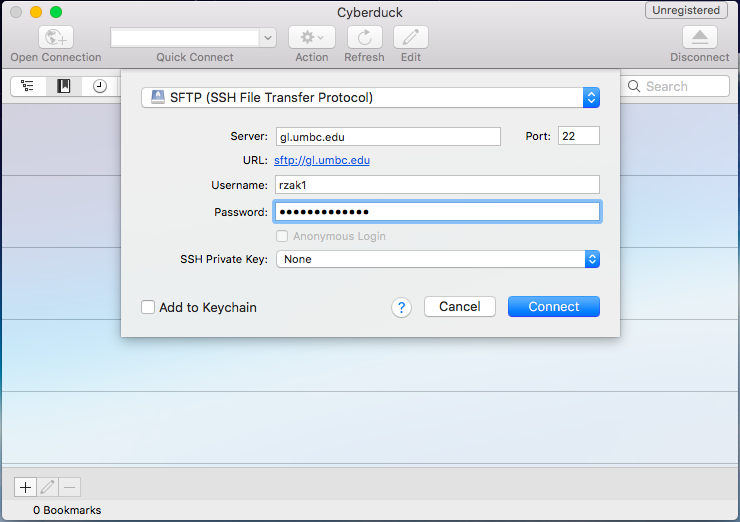
\includegraphics[scale=0.6]{Images/macos_cyberduck_connect.png}
\caption{Connecting to GL with CyberDuck.}
\label{fig:maccyberduckconnect}
\end{figure}

\begin{figure}
\centering
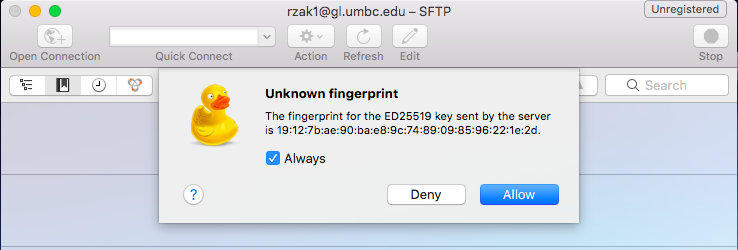
\includegraphics[scale=0.6]{Images/macos_cyberduck_firsttime.png}
\caption{CyberDuck asking about the server's SSH key.}
\label{fig:maccyberduckconnectfirsttime}
\end{figure}

\begin{figure}
\centering
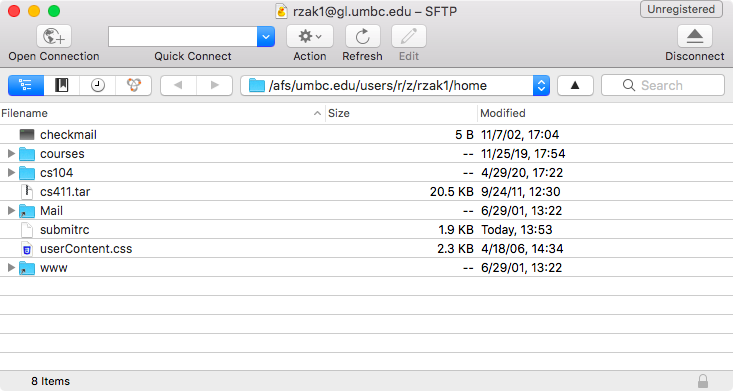
\includegraphics[scale=0.6]{Images/macos_cyberduck_connected.png}
\caption{CyberDuck asking about the server's SSH key.}
\label{fig:maccyberduckconnected}
\end{figure}

\FloatBarrier
\section{Extras}
\subsection{Shortcuts}
\paragraph{}Left as an exercise to the reader, Putty, WinSCP, and CyberDuck allow shortcuts. This allows you to easily reconnect to the UMBC GL servers without having to re-type the server name and your credentials.

\subsection{SSH Keys}
\paragraph{}Even after connecting for the first time, you may get a message about accepting SSH keys. This is expected for two reasons:

\begin{enumerate}
    \item The GL system consists of a few different Linux servers, and the GL system decided at connect time which one you'll be connecting to. For our purposes, it doesn't matter which you use, as they all will have your files, and all contain the programs we need.
    \item Sometimes, especially after an update on the server side, the SSH keys may change. It's not a cause for concern.
\end{enumerate}

\end{document}